%!TEX root = ../main.tex

\section{Selection (5 pages)}
\label{sec:b02dd:selection}

The amount of background in \BdToDD is too high to perform a significant
measurement of \CP violation without any selection. The selection is divided
into three parts: a preselection with many high signal efficiency
requirements, a dedicated treatment of mis-identified backgrounds and a
multivariate analysis to further reduce combinatorial background.

\subsection{Preselection}
\label{sec:b02dd:selection:cuts}

\todo{Preselection for \BdToDD}

\subsection{Vetoes}
\label{sec:b02dd:selection:vetoes}

A $K\rightarrow\pi$ mis-ID can lead to background contributions from
$\DspToKKpi$, which predominantly proceeds through $\DsTophipi$. To reduce
these $\Dsp$ contributions the kaon mass hypothesis is assigned to the pion
with the higher transverse momentum of $\DpToKpipi$ candidates. The candidate
is rejected if the invariant mass of the hypothetical kaon pair is compatible
with the $\phi$ mass of $M_{\phi} = \SI{1019.461}{\MeVcc}$~\cite{PDG2014}
within $\pm\SI{10}{\MeVcc}$ or if the invariant mass $m(\Km\Kp\pip)$ is
compatible with the \Dsp mass of $M_{\Dsp} =
\SI{1968.30}{\MeVcc}$~\cite{PDG2014} within $\pm\SI{25}{\MeVcc}$ and the pion
with the higher \pT (the one that the kaon mass hypothesis is assigned to) has
a larger $\texttt{ProbNN}K$ than $\texttt{ProbNN}\pion$ probability. When
assigning the kaon mass hypothesis to the pion with the lower \pT no vetoes
are applied as no resonant structures at the $\phi$ or the $\Dsp$ mass are
found.

To reduce $p\rightarrow\pi$ mis-ID the proton mass hypothesis is assigned to
the pion with the higher \pT of $\DpToKpipi$ candidates. The candidate is
rejected if the invariant mass of the $\kaon\proton\pion$ combination is
compatible with the \Lc mass of $M_{\Lc} =
\SI{2286.46}{\MeVcc}$~\cite{PDG2014} within $\pm\SI{25}{\MeVcc}$ and the
proton probability $\texttt{ProbNN}p$ of the pion with the higher \pT is
larger than $\texttt{ProbNN}\pion$.

\subsection{Multivariate analysis}
\label{sec:b02dd:selection:mva}

\subsubsection{Training of a BDT}
\label{sec:b02dd:selection:mva:training}

To further suppress combinatorial background a Boosted Decision Tree
(BDT)~\cite{Breiman,Roe} based on the implementation in
TMVA~\cite{Hocker:2007ht} is trained using a signal MC sample and the upper
mass sideband with $m_{\Dp\Dm} > \SI{5500}{\MeVcc}$. The training is performed
on half of these samples while the other half is used to test the BDT
performance. The selection steps described above, are applied before the
training.

Two BDTs separated by the number of kaons in the \Bd final state are trained.
The importance of the \num{21} input variables to the training differs which
is considered by their order in \cref{tab:b02dd:selection:mva:inputs}.
%
\begin{table}[!htb]
\centering
\caption{List of input variables used in the training of the BDTs.}
\begin{tabular}{ll}
 \toprule
  BDT for \KpipiKpipi                          &  BDT for \KKpiKpipi                           \\
\midrule
  min(\Dpm $\tau$ significance)                &  PID ratio of \Kpm                            \\
  $B$ direction angle                          &  $B$ direction angle                          \\
  $\log($DTF $\chi^2$/ndof$)$                  &  PID ratio of \Kp                             \\
  PID ratio of \Km                             &  $\log($DTF $\chi^2$/ndof$)$                  \\
  PID ratio of \Kp                             &  PID ratio of \Km                             \\
  min \pT of \Kpm                              &  min(\Dpm $\tau$ significance)                \\
  $\log(B$ impact parameter $\chi^2)$          &  $\log($min($h$ Velo $\chi^2$/ndof)$)$        \\
  $\log($min(\pipm Velo $\chi^2$/ndof)$)$      &  \pT of \Kpm                                  \\
  \pT of \pim with lower \pT                   &  $\log($min(\Kpm T-track $\chi^2$/ndof)$)$    \\
  $\log($min(\Kpm T-track $\chi^2$/ndof)$)$    &  $\log(B$ impact parameter $\chi^2)$          \\
  $\log($min(\pipm T-track $\chi^2$/ndof)$)$   &  PID ratio of \pipm with lower \pT            \\
  PID ratio of \pim with higher \pT            &  $\log($min($h$ VELO-T-Match $\chi^2$)$)$     \\
  \pT of \pip with lower \pT                   &  $\log($min(\Kpm Velo $\chi^2$/ndof)$)$       \\
  PID ratio of \pim with lower \pT             &  PID ratio of single \pipm                    \\
  PID ratio of \pip with higher \pT            &  \pT of \pipm with higher \pT                 \\
  \pT of \pip with higher \pT                  &  $\log($min($h$ T-track $\chi^2$/ndof)$)$     \\
  PID ratio of \pip with lower \pT             &  \pT of \pipm with lower \pT                  \\
  $\log($min($\Kpm$ Velo $\chi^2$/ndof)$)$     &  min \pT of \Kp and \Km                       \\
  $\log($min(\pipm VELO-T-Match $\chi^2$)$)$   &  \pT of single \pipm                          \\
  $\log($min($\Kpm$ VELO-T-Match $\chi^2$)$)$  &  $\log($min($\Kpm$ VELO-T-Match $\chi^2$)$)$  \\
  \pT of \pim with higher \pT                  &  PID ratio of \pipm with higher \pT           \\
\bottomrule
\end{tabular}
\label{tab:b02dd:selection:mva:inputs}
\end{table}
%
One of the input variables is the ratio of the kaon over the sum of the kaon and the
pion probabilities:
%
\begin{equation}
\text{PID ratio} = \frac{\texttt{ProbNN}K}{\texttt{ProbNN}K + \texttt{ProbNN}\pion} \, .
\label{eq:b02dd:selection:pidratio}
\end{equation}
%
It turns out that this ratio performs a little bit better than just using the
simple ProbNN variables. Among the other input variables are observables
related to the kinematics of the decay like transverse momenta, decay time
significances and direction angles, qualities of the track segments in the
VELO and the T-stations, and vertex qualities.

Before the training the input variables are transformed to decorrelate and
decompose them into the principal components which improves the performance of
the BDT. The BDTs are each built out of \num{700} trees. The depth of the trees is
limited to three. At each node at least \SI{3}{\percent} of the training
events have to be present. The variables are scanned at \num{40} points to
find the optimal cut value. For the boosting the AdaBoost
method~\cite{AdaBoost} with a boost factor of $\beta = \num{0.1}$ is deployed.

Overtraining is checked by applying the BDT on both the training and the
testing sample (see \cref{fig:b02dd:selection:mva:overtraining}).
%
\begin{figure}[!htb]
\centering
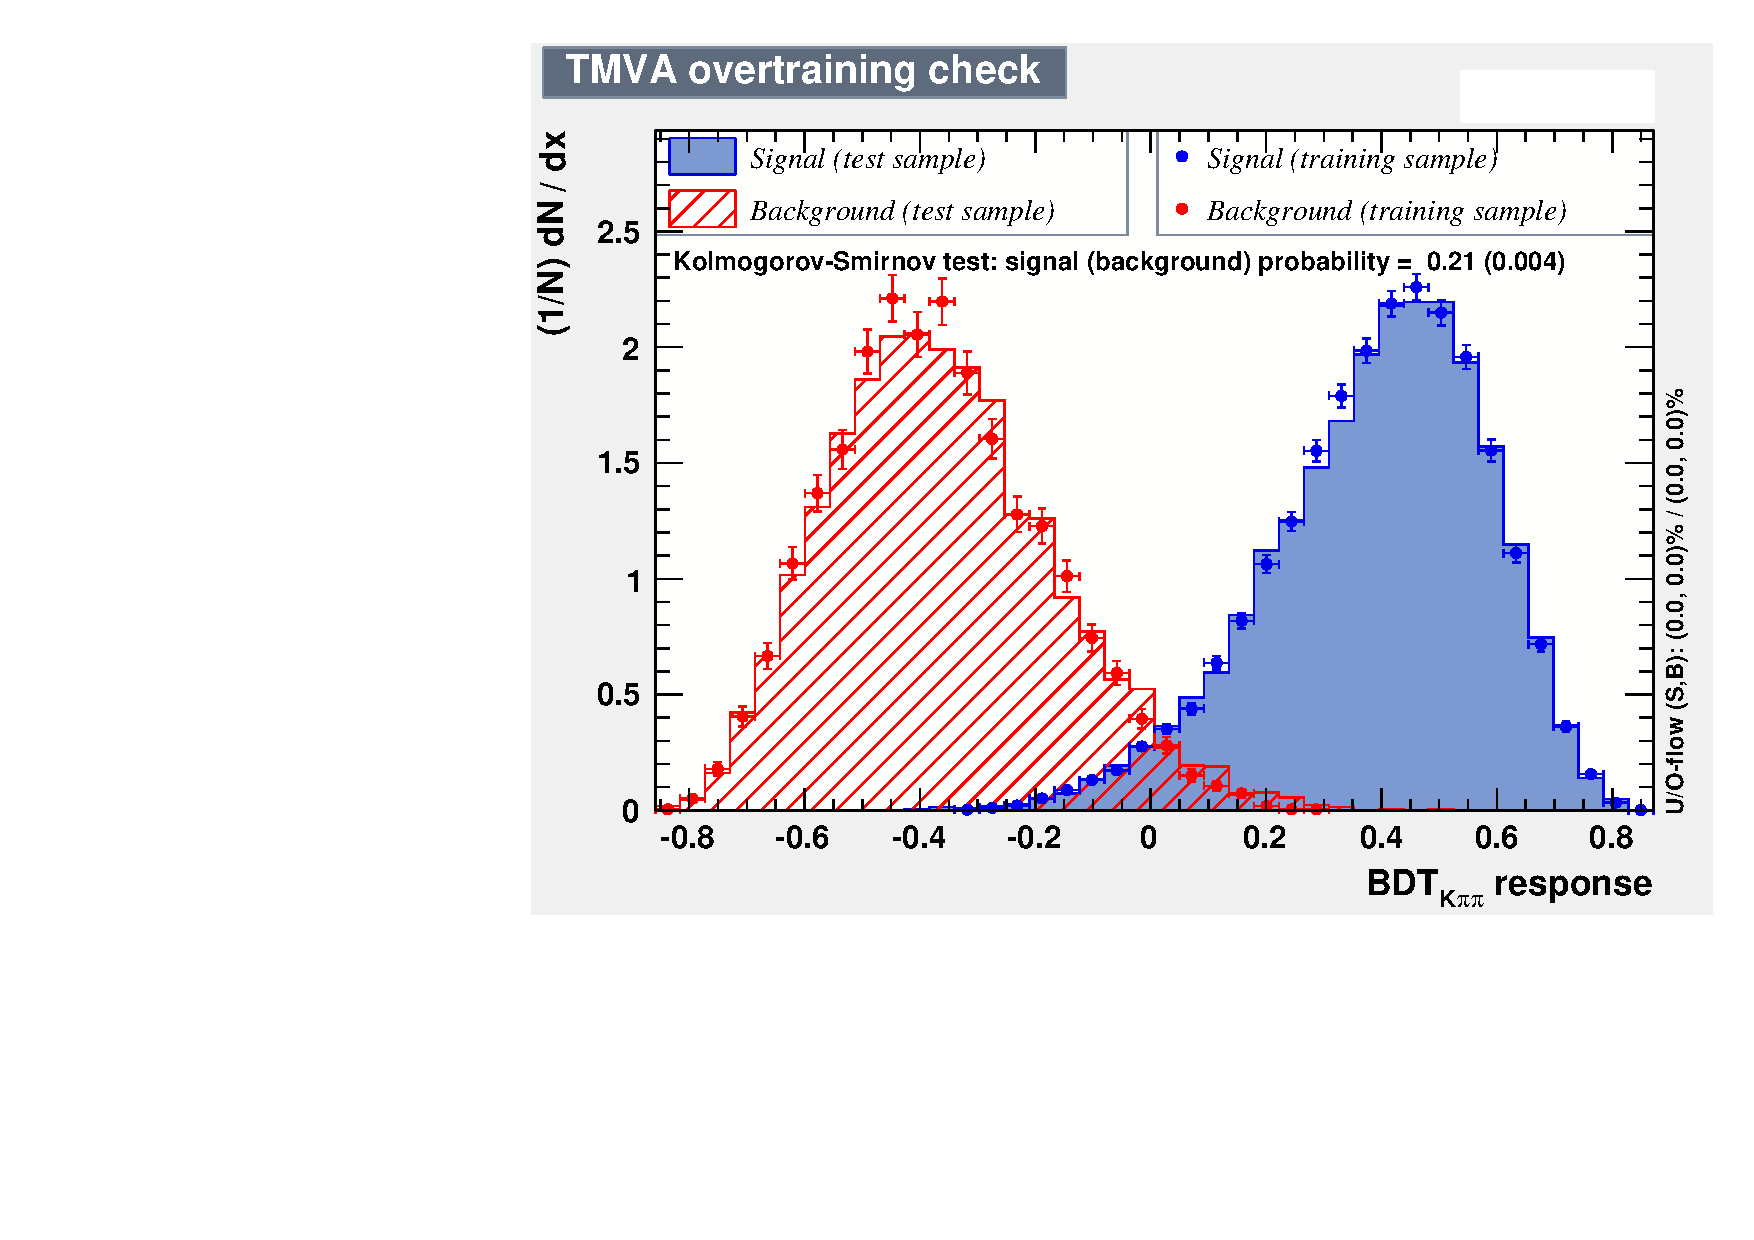
\includegraphics[width=0.48\textwidth]{07-B02DD/figs/Overtraining_Check_Kpipi.pdf}
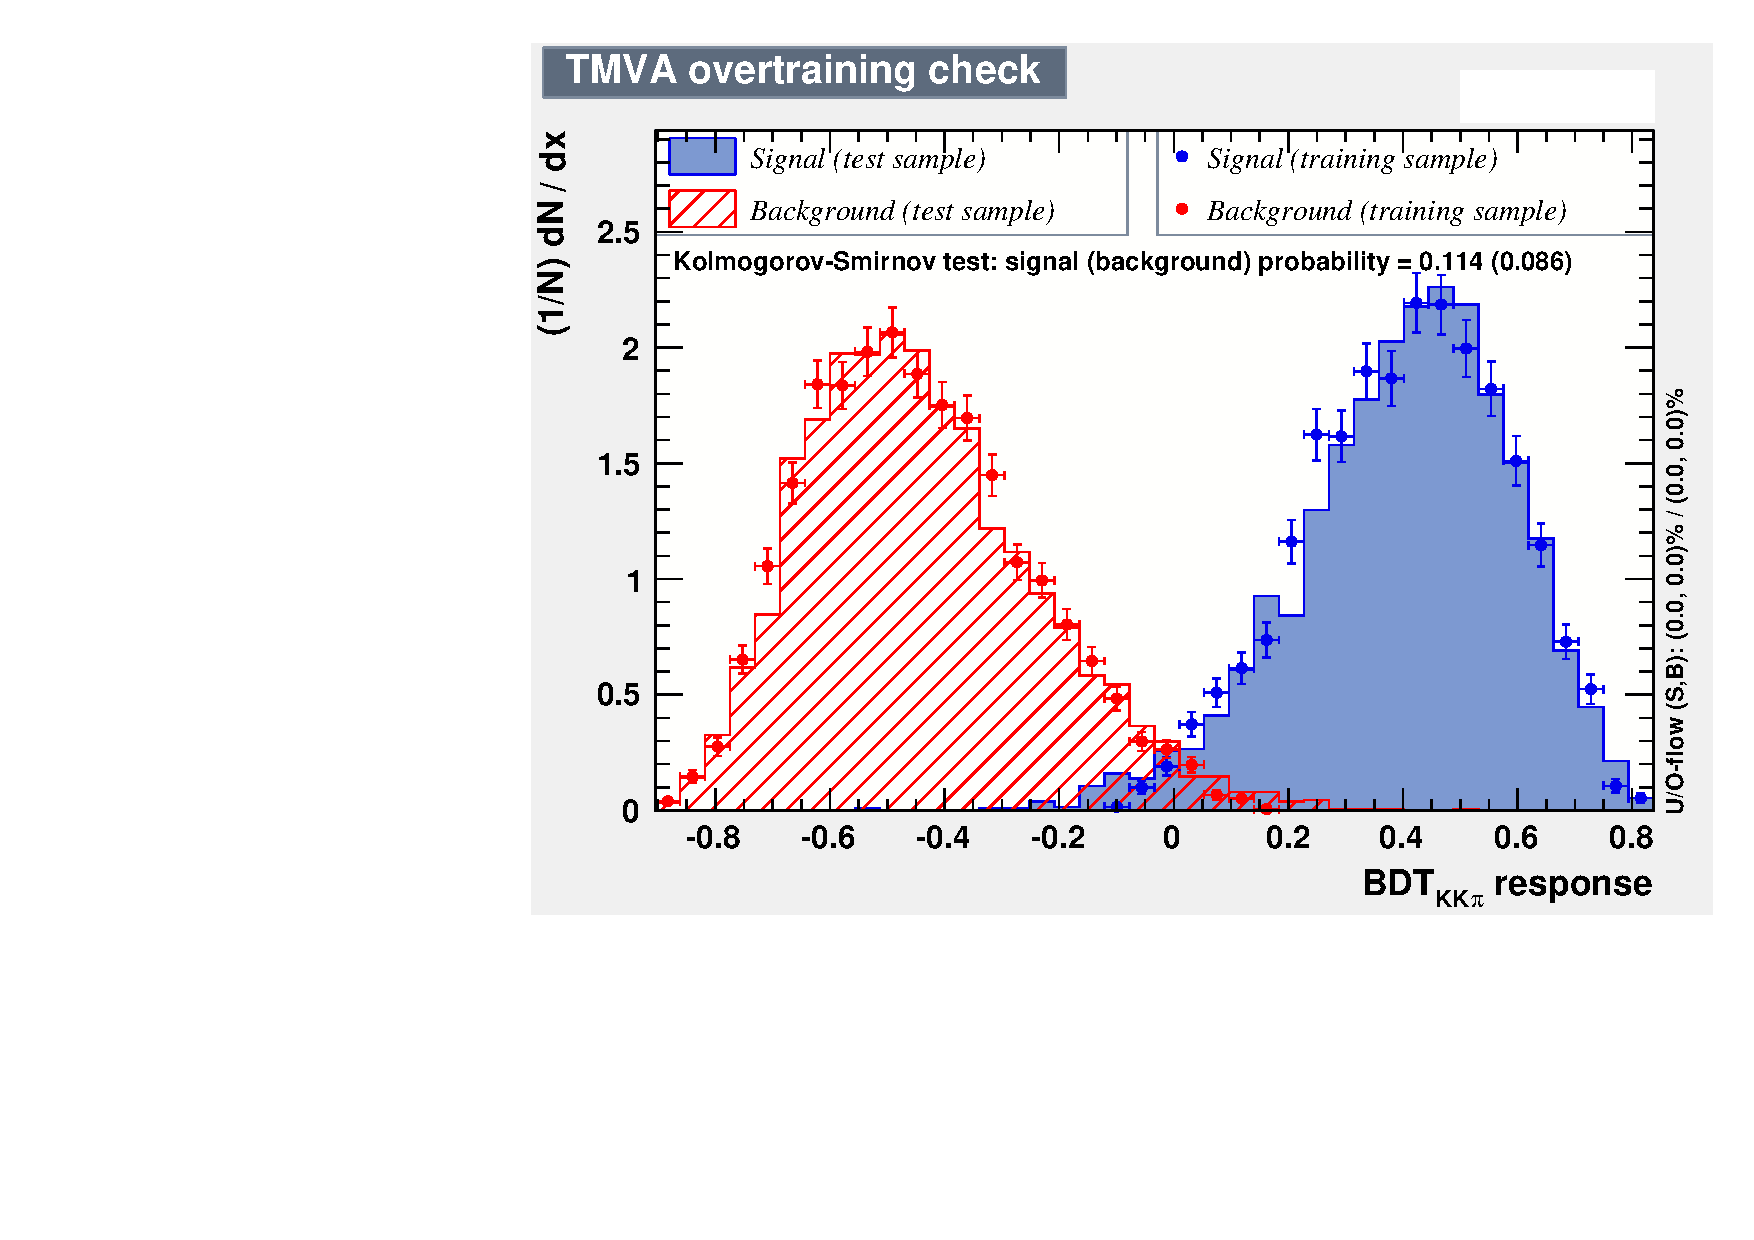
\includegraphics[width=0.48\textwidth]{07-B02DD/figs/Overtraining_Check_KKpi.pdf}
\caption{Comparison of the BDT response on training and test sample for the
\KpipiKpipi final state (left) and the \KKpiKpipi final state (right).}
\label{fig:b02dd:selection:mva:overtraining}
\end{figure}
%
Using simulations in the selection contains the possibility that certain
distributions are not modelled properly and differences between the simulation
and real data are exploited instead of differences between signal and
background. Indeed, the classifier output distributions of the signal MC and
background-subtracted data show a quite large disagreement for both final
states as can be seen in \cref{fig:b02dd:selection:mva:bdtcomparison}. The
performance is clearly overestimated in the training.
%
\begin{figure}[htbp]
    \centering
    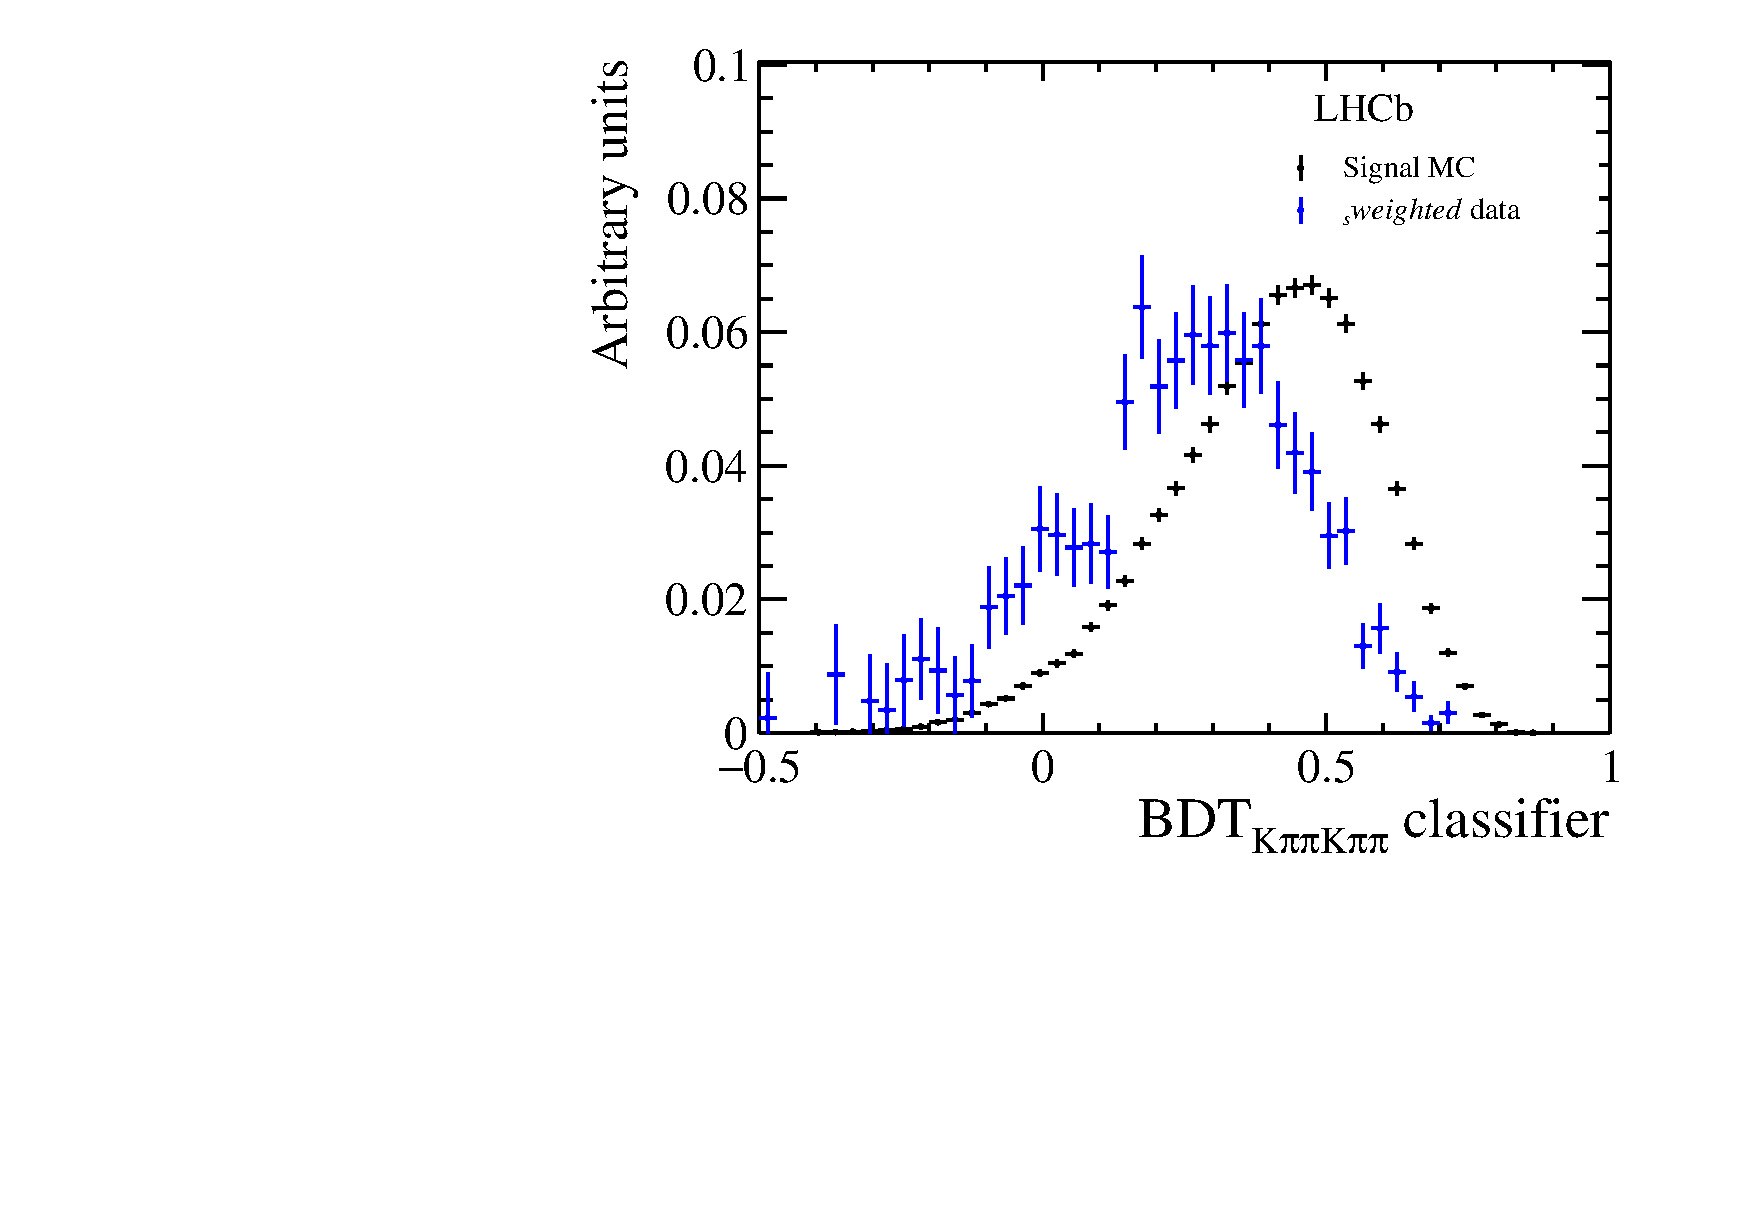
\includegraphics[width=0.49\textwidth]{07-B02DD/figs/BDTComparison_Kpipi.pdf}
    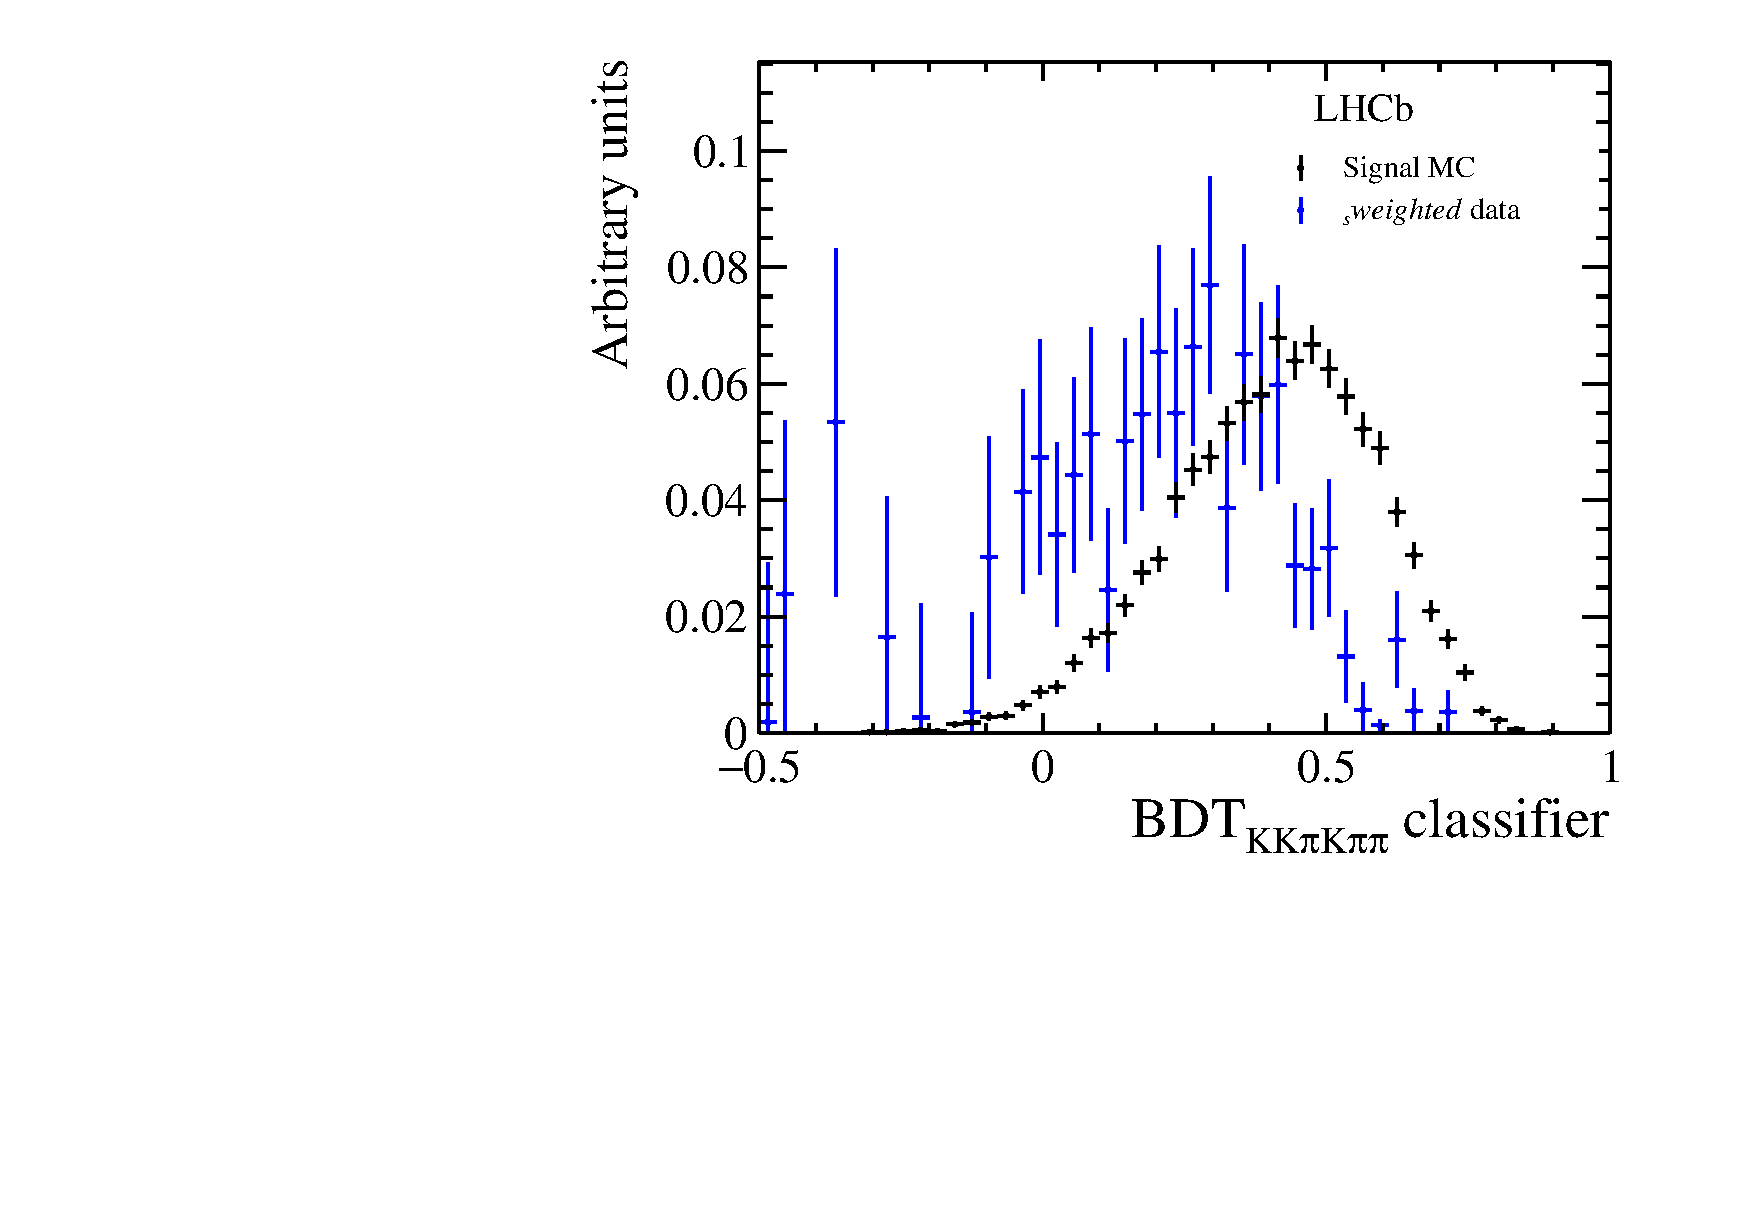
\includegraphics[width=0.49\textwidth]{07-B02DD/figs/BDTComparison_KKpi.pdf}
    \caption{Distribution of the BDT output for background-subtracted data (blue) and
    signal MC (black) for the \KpipiKpipi final state (left) and the
    \KKpiKpipi final state (right).}
    \label{fig:b02dd:selection:mva:bdtcomparison}
\end{figure}
%
This would be a problem if the selection efficiencies had to be calculated
using the MC sample. But for a measurement of \CP violation it is mainly
important that the amount of background can somehow be reduced while most of
the signal is kept. This can be achieved with the current setting.

% ==============================================================================
\subsubsection{BDT cut optimisation}
\label{sec:b02dd:selection:mva:optimisation}

As explained in \cref{sec:dataanalysis:selection:fom} the best figure of merit
for a measurement of \CP violation is the sensitivity on the \CP observables
themselves. So the requirement on the BDT classifier output is scanned
performing a fit to the invariant $\Dp\Dm$ mass spectrum followed by a decay
time fit of the background-subtracted sample for each scan point. Initially,
only the subsample with two kaons in the \Bd final state is analysed. In
\cref{fig:b02dd:selection:mva:sensitivities} the statistical
uncertainties of \SDD and \CDD are plotted as a function of the requirement on
the BDT classifier output.
%
\begin{figure}[!htb]
\centering
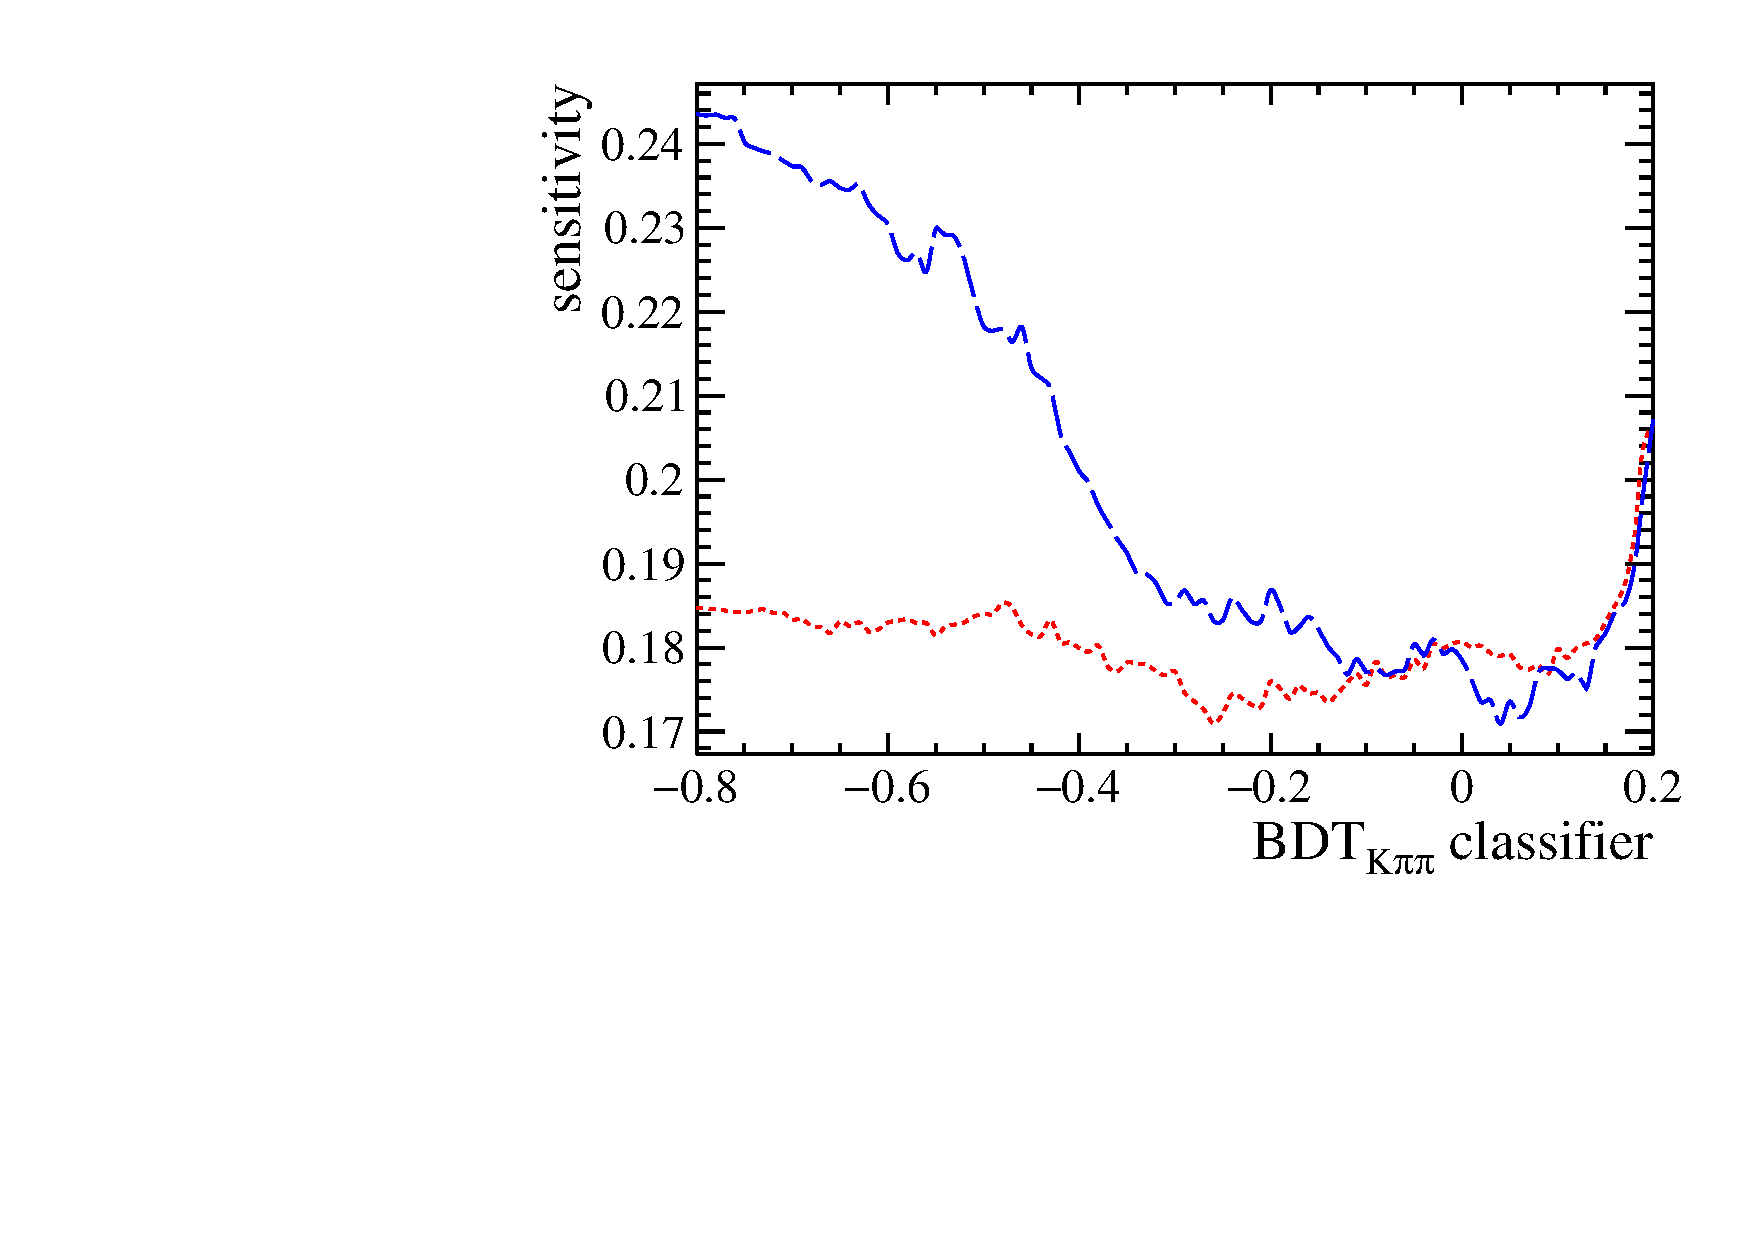
\includegraphics[width=0.48\textwidth]{07-B02DD/figs/Sensitivities_Kpipi.pdf}
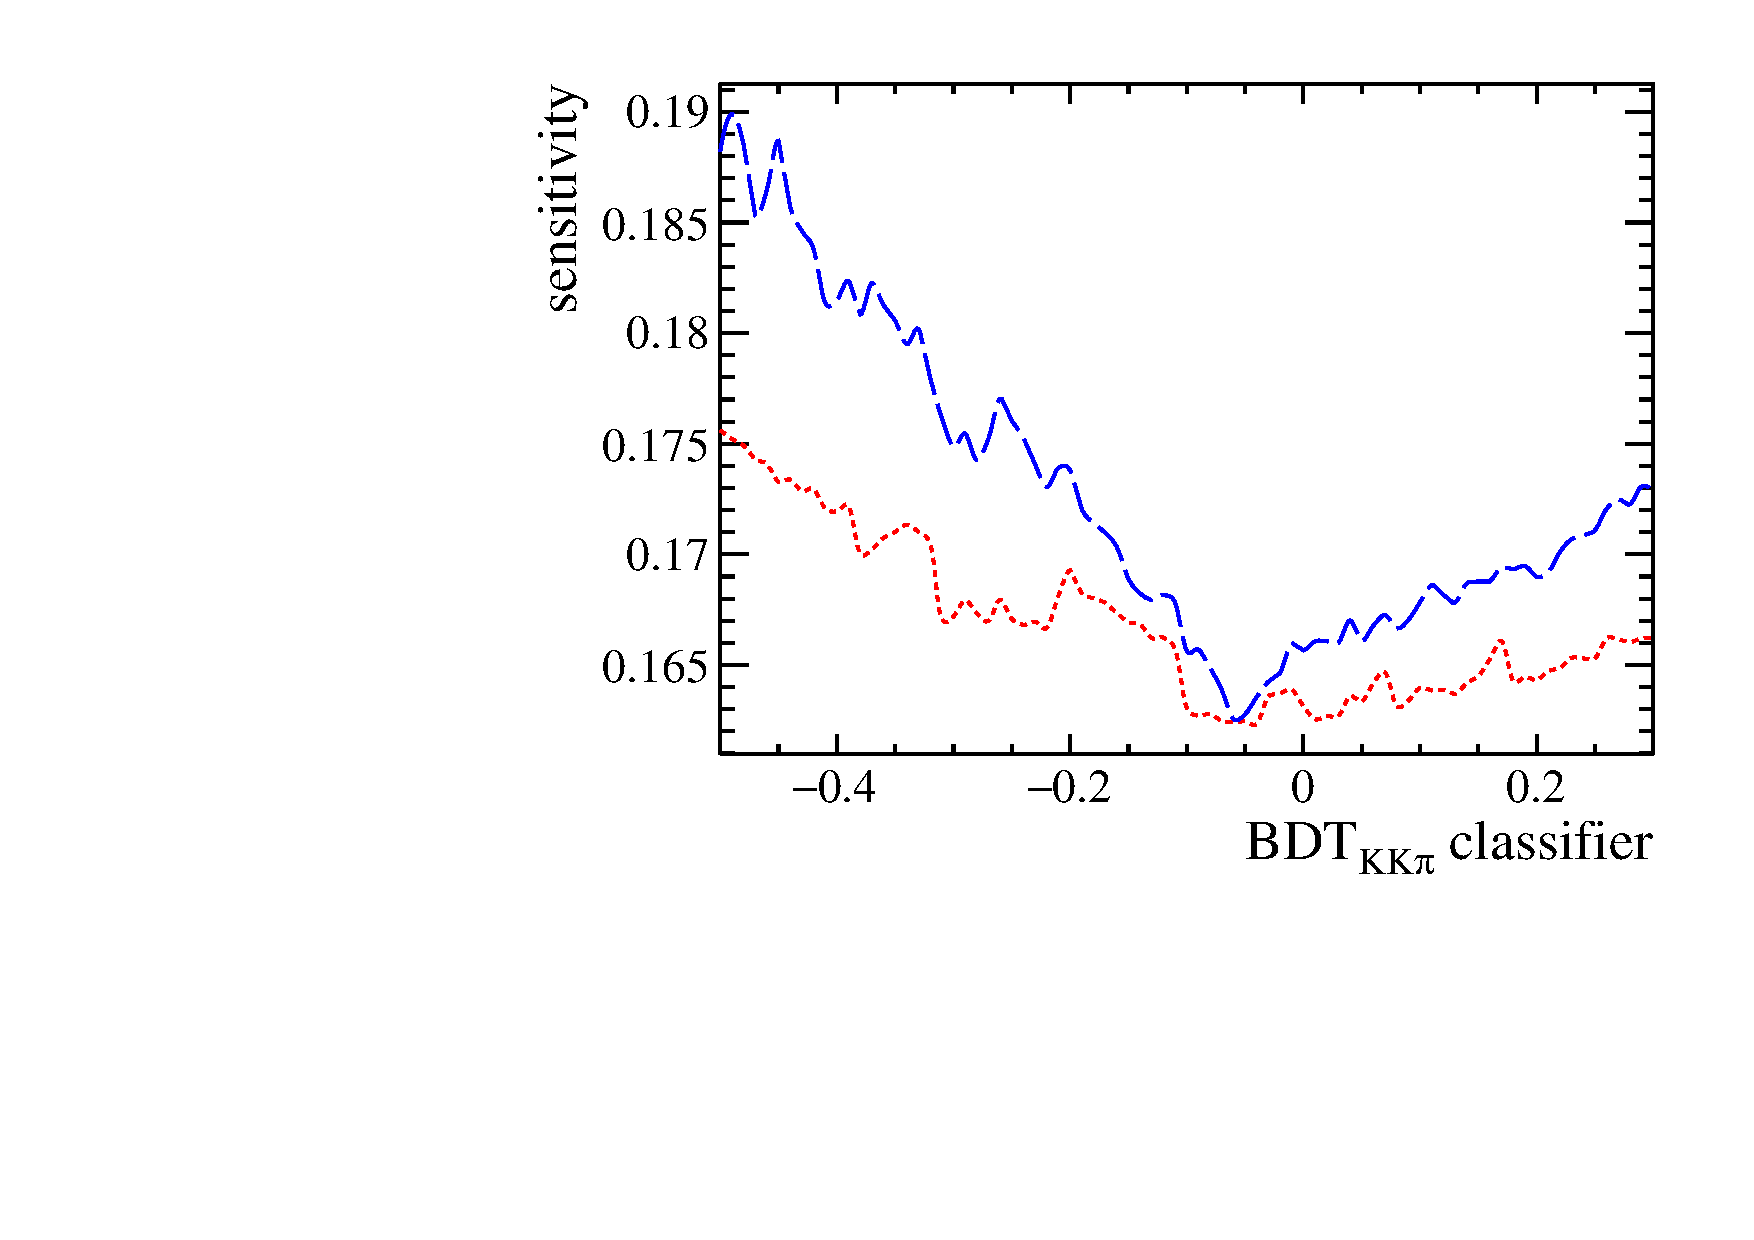
\includegraphics[width=0.48\textwidth]{07-B02DD/figs/Sensitivities_KKpi.pdf}
\caption{Sensitivity of \SDD (red short-dashed) and \CDD (blue long-dashed) as
a function of the BDT classifier output for the \KpipiKpipi final state (left)
and the \KKpiKpipi final state (right).}
\label{fig:b02dd:selection:mva:sensitivities}
\end{figure}
%
The uncertainty on \CDD improves with tighter requirements on the BDT
classifier until it reaches an optimum shortly after zero. This can be
explained with the fact that the sensitivity on \CDD mainly comes from
candidates at low decay times because the cosine function is maximal there.
The suppression of the rather short-lived combinatorial background compensates
the loss in signal efficiency for a quite long range. In contrast, the
uncertainty on \SDD is mainly driven by the amount of signal candidates. So it
is more or less flat for loose requirements on the BDT classifier where only
few signal candidates are lost and this is compensated by the higher purity
and reaches its optimum around \num{-0.25} before it starts to get worse. Now
that both observables are of interest and the optima are not at the same cut
value it is decided to require the BDT classifier to be greater than
\num{-0.10}. This is a good compromise between both observables as the
uncertainties of \SDD and \CDD are almost the same and close to their optima.
The requirement has a signal efficiency of \SI{96.5\pm0.5}{\percent} and
rejects \SI{84.18\pm0.34}{\percent} of the combinatorial background.

In a second step the requirement on the BDT classifier for the \KKpiKpipi
final state is optimised. The \KKpiKpipi subsample is quite small which makes
individual fits on this subsample rather unstable. This can be solved by
performing a simultaneous fit to the whole dataset with the previously
determined BDT cut applied to the \KpipiKpipi subsample. Scanning the BDT
classifier output for the \KKpiKpipi final state results in the sensitivities
on \SDD and \CDD plotted in \cref{fig:b02dd:selection:mva:sensitivities}. Both
uncertainties show a minimum at around \num{-0.05} which is chosen as cut
value. This cut removes \SI{90.75\pm0.33}{\percent} of the combinatorial
background at a signal efficiency of \SI{87.2\pm1.9}{\percent}.

\clearpage
